%-----------------------------------------------------------------
%	LA NOSTRA GALÀXIA: LA VIA LÀCTIA
%	!TEX root = ./../main.tex
%-----------------------------------------------------------------
\section{La nostra galàxia: la Via Làctia}
\subsection{Forma i mida de la Via Làctia}
La majoria d'estrelles visibles a simple vista de la nostra galàxia (la Via Làctia, o simplement la Galàxia) es troba en un gegant disc prim (figura \ref{fig:disc}).
\begin{figure}[h]
	\centering
	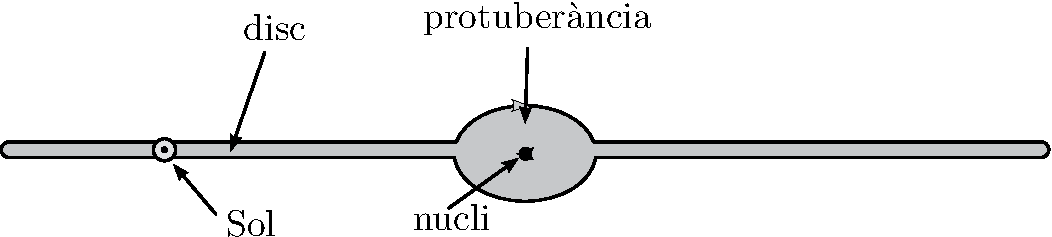
\includegraphics[width=0.7\textwidth]{./images/6-disc}
	\caption{La nostra posició a la Galàxia. Som al centre del disc, però més lluny del centre de la Galàxia que de l'extrem del disc}
	\label{fig:disc}
\end{figure}

El disc el veiem de cantonada, ja que ens trobem en ell; a l'estiu (hemisferi nord), destaca més que a l'hivern (figura \ref{fig:disc-nord-sud}).
\begin{figure}[h]
	\centering
	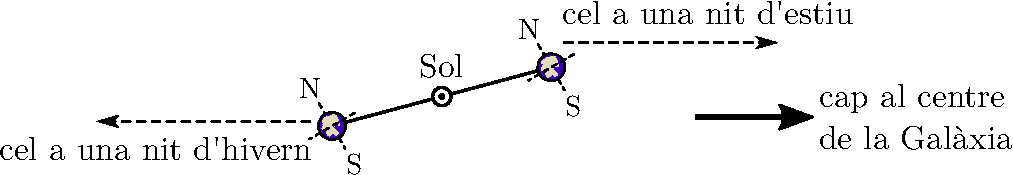
\includegraphics[width=0.8\textwidth]{./images/6-disc-nord-sud}
	\caption{Un observador a l'hemisferi nord veu amb major prominència el disc de la Galàxia a l'estiu que a l'hivern}
	\label{fig:disc-nord-sud}
\end{figure}

\subsubsection*{Univers de Kapteyn}
Inicialment es creia que el sistema solar es trobava al centre de la Via Làctia. Efectivament, si comptem el nombre d'estrelles de diferent magnitud aparent en cada direcció del cel i suposem que la densitat numèrica d'estrelles de lluminositat $L$ no canvia amb la posició, $n(L) = cte$, es dedueix que el nombre d'estrelles amb magnitud aparent major que cert valor llindar $F_{0}$, ve donat per
\begin{align}\label{eq:dens-estrelles}
	N(F > F_{0}) = \frac{A}{F_{0}^{3/2}} \qc \text{on } A = cte
\end{align}
% \begin{sproof}
%     TODO: demostració a classe
% \end{sproof}

Aquesta equació implica que si es troben 1000 estrelles amb $F>F_{0}$ duen haver 8000 estrelles amb $F/F_{0}/4$ (l'augment és degut al fet que quan es consideren valors de $F$ menors estem incloent estrelles més llunyanes).

El que en realitat es va trobar és que el nombre d'estrelles no creix tan ràpid en disminuir $F_{0}$. Ja que la fórmula \eqref{eq:dens-estrelles} es basa en suposar que les estrelles estarien distribuïdes uniformement, es va arribar a la conclusió (falsa) que la distribució d'estrelles decreix amb la distància al nostre sistema solar. Per tant, hauríem d'estar a prop del centre de la distribució d'estrelles al cel. A més, al decaure el nombre d'estrelles més ràpidament en unes direccions que altres es va pensar que hauríem d'estar a prop d'una \textit{distribució plana d'estrelles fixes}, en què el gruix de la Via Làctia seria aproximadament $1/5$ del seu diàmetre (vegeu la figura \ref{fig:kapteyn}, la qual mostra l'Univers de Kapteyn (1851--1922)).
\begin{figure}[h]
	\centering
	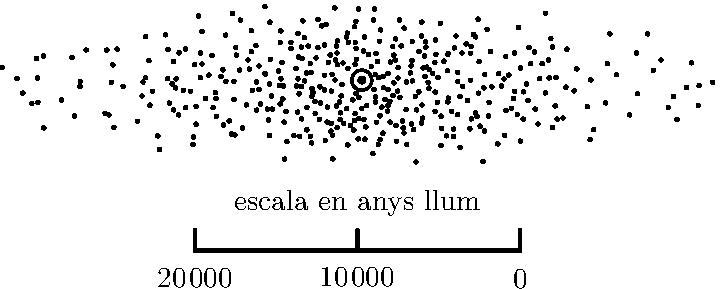
\includegraphics[width=0.7\textwidth]{./images/6-kapteyn}
	\caption{Escala i forma de l'Univers de Kapteyn. El Sol està situat al centre del sistema d'estrelles; l'amplada d'aquest és $\approx 1/5$ del seu radi}
	\label{fig:kapteyn}
\end{figure}

\subsubsection*{Univers de Shapley}
%FIXME: shapley@sec:bio
Harlowe Shapley (1885--1972) va demostrar que aquest univers era erroni. Shapley va utilitzar les estrelles polsants RR Lyrae (la lluminositat variable de les quals les fa destacar) per determinar la distància que ens separa dels cúmuls globulars (que posseeixen RR Lyrae) i va advertir que es distribuïen 2000, aproximadament, amb simetria més o menys esfèrica en torn al centre del disc (no ocupat pel Sol).

Desconeixent la presència de pols al mitjà interestel·lar va sobreestimar les distàncies. No obstant, aquesta descripció és acceptada avui (figura \ref{fig:shapley}).

Els cúmuls globulars se situen bàsicament en l'halo, per això l'extinció per la pols (situada preferentment al disc) afecta poc a la seva lluminositat.

D'aquest anàlisi va resultar que el Sol es troba a uns 25 mil anys llum ($\approx \SI{8}{\kilo\parsec}$) del centre de la Galàxia. Per estudiar el centre de la Galàxia s'ha de recórrer a longituds d'ona típiques de raigs X i raigs gamma. Aquests revelen que esdeveniments altament energètics tenen lloc allà.

El treball de Shapley i l'estudi de la galàxia M31 (Andròmeda) per Walter Baade (1893--1960) va mostrar que la distribució espacial d'estrelles riques en metalls (població I) difereix de la distribució espacial d'estrelles pobres en metalls (població II). Les estrelles al disc són bàsicament de població I; a la protuberància es dóna una barreja d'ambdues poblacions, i en l'halo pràcticament totes són de la població II.

Avui es coneix que la lluminositat del disc és $\approx \SIrange{15}{20}{\Lsun}$, i la de la protuberància és $\approx \SI{5 e9}{\Lsun}$. La massa del disc en estrelles és $\approx \SI{60 e9}{\Msun}$, i la de la protuberància $\approx \SI{20 e9}{\Msun}$. Les estrelles de l'halo contribueixen amb només $\SI{e9}{\Msun}$ a la massa de la Galàxia.
\begin{figure}[ht]
	\centering
	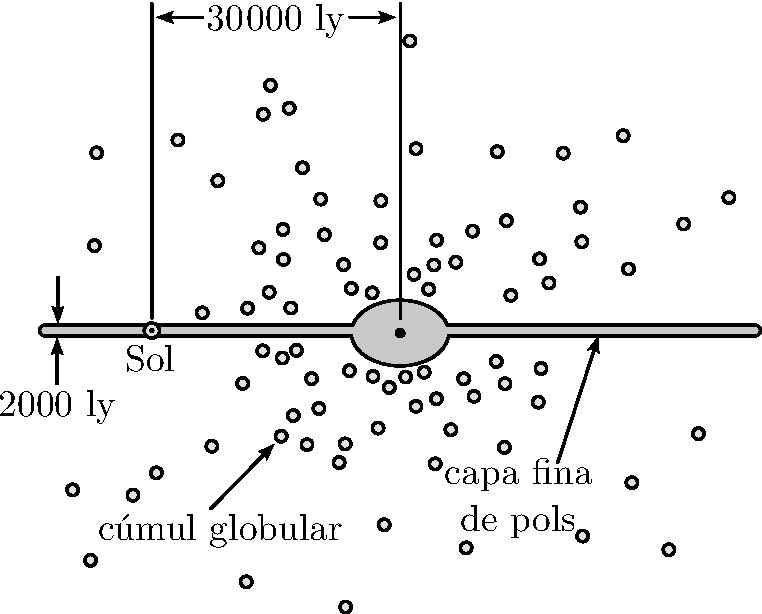
\includegraphics[width=0.55\textwidth]{./images/6-shapley}
	\caption{Visió actual de l'estructura de la Galàxia. Es composa d'un disc prim d'estrelles, gas i pols, una protuberància central, i un halo d'estrelles velles}
	\label{fig:shapley}
\end{figure}

\subsubsection*{Moviment i forma de la galàxia}
El moviment de les estrelles i núvols de gas a la nostra galàxia explica a grans trets la forma d'aquesta.
\begin{figure}[H]
	\centering
	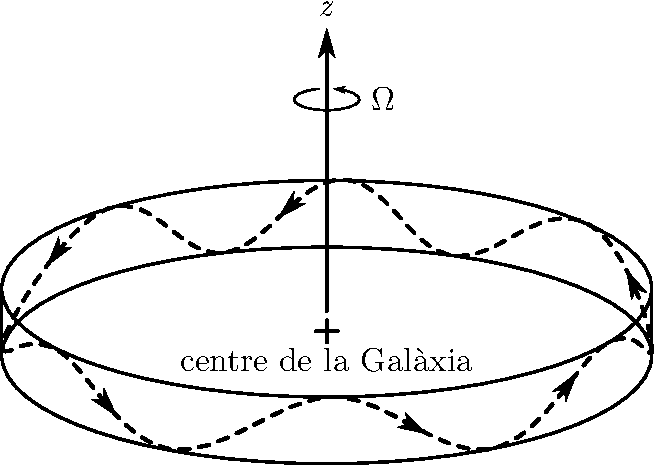
\includegraphics[width=0.5\textwidth]{./images/6-vel-disc}
	\caption{Il·lustració de com la velocitat circular de l'òrbita d'una estrella del disc en ser molt major que la seva velocitat segons l'eix $z$ condueix a que aquestes estrelles donin lloc a una distribució aplanada amb centre al centre de la Galàxia}
	\label{fig:vel-disc}
\end{figure}

El disc està format per estrelles la velocitat de les quals en torn al centre de la Galàxia és molt major que la velocitat del seu moviment erràtic. Això impedeix que col·lapsin a un punt comú i les obliga a romandre al disc (figura \ref{fig:vel-disc}).

La protuberància conté estrelles d'escassa velocitat circular, d'aquesta manera aquestes estrelles formen aproximadament una distribució esfèrica (figura \ref{fig:milky-protuberance}).
\begin{figure}[H]
	\centering
	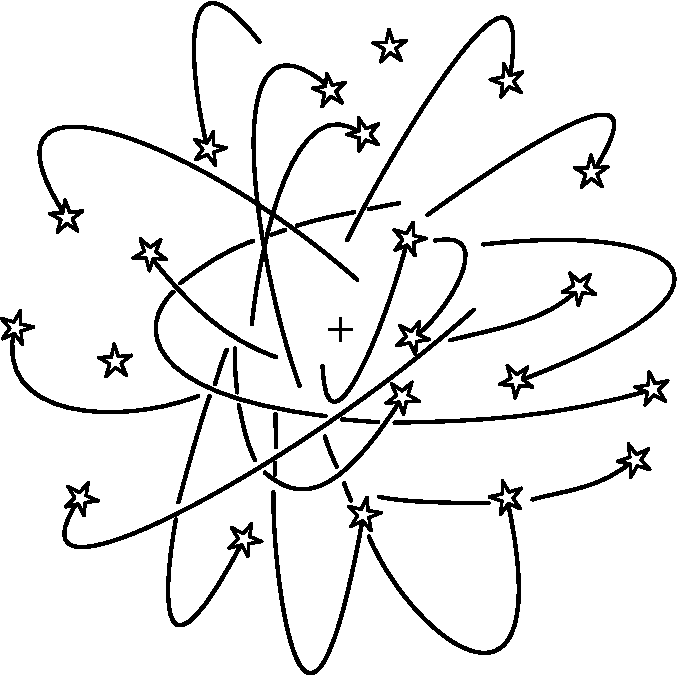
\includegraphics[width=0.5\textwidth]{./images/6-milky-protuberance}
	\caption{La protuberància central està formada per estrelles que no posseeixen una rotació mitjana important. Es mouen en torn al centre $\otimes$ de forma més o menys erràtica donant la impressió (falsa) d'abelles en torn a un rusc. L'equilibri entre el moviment circular i l'atracció gravitatòria cap al centre dóna lloc a la forma esfèrica de la protuberància. La forma exacta d'aquesta no es coneix bé a causa de l'extinció}
	\label{fig:milky-protuberance}
\end{figure}

L'halo està format per estrelles que executen un moviment més o menys harmònic travessant cap a dalt i cap a ball el disc de la Galàxia. La seva component erràtica és clarament major que la de les estrelles del disc i estan menys unides a la Galàxia que les estrelles de la protuberància.

Podria donar-se una transició lenta d'estrelles de la protuberància a l'halo.

%-----------------------------------------------------------------
\subsection{Matèria fosca}
El gruix del disc de la Galàxia al veïnatge del Sol es pot mesurar amb ajuda d'estrelles gegants de tipus espectral K. Aquestes són nombroses i relativament brillants de manera que no són difícils de veure fins i tot a grans distàncies del pla central del disc.

Això, combinat amb mesures de les velocitats erràtiques d'aquestes estrelles, permet deduir la intensitat de la component normal $g_{\perp}$ del camp gravitatori; amb això es pot trobar la massa local necessària per produir aquest camp. A continuació es pot comparar aquesta massa amb la massa observada en forma d'estrelles i núvols de gas.

% FIXME: oort@sec:bio
Per aquest procediment Jan Oort (1895-1965) va descobrir que la massa observada és només la meitat de la requerida per produir aquesta acceleració. Aquesta discrepància és només la primera d'una sèrie detectada en mesures dinàmiques de massa a escala de galàxies i cúmuls de galàxies (el problema de la massa oculta, \textit{missing mass problem}). Se'ns planteja la següent qüestió: existeix potser una massa enorme de matèria no--lluminosa només detectable gràcies a la seva influència gravitatòria?

\subsubsection*{Quocient massa/llum}
Al disc de la Galàxia, al veïnatge del Sol, es té $M/L = 5 \, \Msun/\Lsun$. Aquest valor és també de l'ordre de l'observat en les parts visibles de les galàxies espirals. Això té les següents implicacions:
\begin{enumerate}[(i)]
	\item La massa mitjana de la Galàxia és menys eficaç en produir llum que el Sol. Això es consistent amb el fet que la majoria de les estrelles a la Galàxia són de tipus espectral K febles, o nanes de tipus M, les quals són poc massives (i menys lluminoses que les massives). Hem de concloure, doncs, que la major part de la llum de la Galàxia (excepte en la zona infraroja de l'espectre) procedeix d'un petit nombre d'estrelles massives blaves, i/o de gegants en fase d'evolució avançada. Una fracció important de la massa al disc de la Galàxia està en forma de nanes poc lluminoses i poc massives, i potser en nanes fosques o fins i tot forats negres.
	\item La segona conseqüència es refereix a la producció d'heli. Matèria tan poc eficaç en produir llum no pot haver produït l'heli observat a l'Univers (25\% en massa). El Sol (amb quocient $(M/L)_{\odot} \equiv 1$, per definició) aconsegueix convertir només el 10\% del seu hidrogen en heli en $10^{10}$ anys; de forma que matèria amb $M/L \sim 5$ només convertirà (per processos nuclears) el 2\% del seu hidrogen en heli (en $10^{10}$, aproximadament l'edat de la Galàxia). La major part d'aquest heli es trobaria tancat a l'interior de les estrelles, no incorporant-se a noves generacions d'estrelles; només contribuiria una dècima part a l'heli observat a escales còsmiques.

	Per descomptat, podria ser que els processos nuclears a les estrelles haguessin procedit més ràpidament en temps passats que ara; però els astrònoms creuen que l'heli produït a les estrelles no pot superar en molt 3 cops la producció d'elements pesats (aproximadament 2\% en massa). Així doncs, la major part de l'heli té origen no estel·lar. Molt possiblement va ser produït als primers minuts de l'expansió de l'Univers.
\end{enumerate}

\subsubsection*{Corbes planes de rotació}
Mesures de la línia espectral de $\SI{21}{\cm}$ de l'hidrogen neutre (H I), a causa de l'spin-flip de l'electró, han permès determinar empíricament les corbes de rotació, $v = v(r)$, en més de 100 galàxies espirals.
\begin{figure}[h]
	\centering
	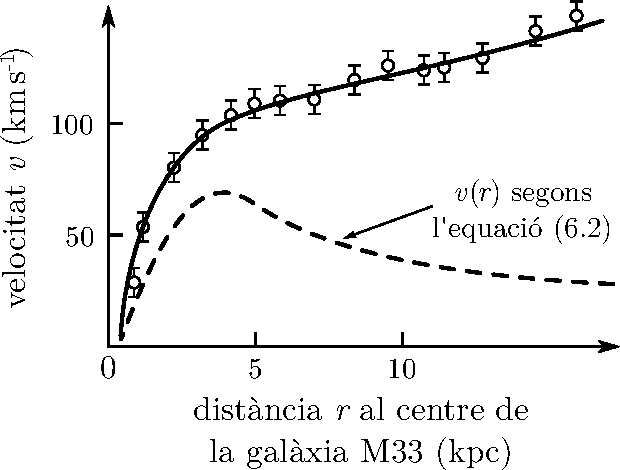
\includegraphics[width=0.5\textwidth]{./images/6-rotation-curve}
	\caption{La corba de rotació de la galàxia espiral nana M33 s'estén molt més enllà de la seva imatge òptica}
	\label{fig:rotation-curve}
\end{figure}

A partir de $\displaystyle m \frac{v^{2}(r)}{r} = G \frac{m M(r)}{r^{2}}$ sobté que la corba de rotació hauria de complir
\begin{align}\label{eq:vel-rotacio}
	v(r) = \sqrt{G \frac{M(r)}{r}}
\end{align}
no obstant els resultats empírics esmentats indiquen una massa molt major que l'observada visualment (matèria fosca). És a dir, la massa de les galàxies segueix creixent molt més enllà tot i que no hi hagi component lluminosa que provoqui aquest augment (figura \ref{fig:rotation-curve}).

Els resultats indiquen que $M/L \approx \SIrange{10}{20}{\Msun/\Lsun}$ a galàxies el·líptiques i espirals; $M/L \approx \SIrange{200}{600}{\Msun/\Lsun}$ a galàxies de baixa lluminositat superficial i a galàxies nanes. En el cas de la galàxia M33 (una galàxia espiral a $\SI{3 e6}{\lightyear}$ de la Via Làctia; [\href{http://apod.nasa.gov/apod/ap030924.html}{APOD~030924}]), es troba que $(M/L)_{Draco} = \SI{440 \pm 240}{\Msun/\Lsun}$.

\subsubsection*{Matèria fosca en cúmuls de galàxies}
Per a cúmuls de galàxies que han assolit l'equilibri dinàmic, el teorema virial
\begin{align}\label{eq:thm-virial}
	K + \frac{1}{2} U = 0
\end{align}
relaciona l'energia cinètica del cúmul $K \approx (3/2) M \ev{v_{r}^{2}}$, on $\ev{v_{r}^{2}}^{1/2}$ és la dispersió de velocitat en la visual, amb l'energia potencial mitjana del cúmul $U \approx - G M^{2}/R$, essent $R$ la mida del cúmul (cúmuls al Catàleg d'Abell solen tenir $R \approx \SI{2.15}{\mega\parsec}$).

La relació \eqref{eq:thm-virial} ens permet determinar l'energia potencial (si la cinètica es coneix amb certa precisió) i d'aquesta deduir la massa gravitatòria del cúmul. El quocient $M/L$ pot arribar a ser tan gran com $\SI{300}{\Msun/\Lsun}$. No obstant això, com que la major part de la massa als cúmuls està en forma de gas calent emissor de raigs X, s'estima que $M/M_{lluminosa} \approx 20$, on $M_{lluminosa}$ és la massa total de matèria lluminosa (incloent-hi estrelles i gas).

Al 1933 Fritz Zwicky (1898--1974) va advertir que les velocitats de les galàxies individuals al Cúmul de Coma eren molt grans, i que aquest cúmul podria romandre lligat gravitacionalment només si la seva massa total excedís substancialment la suma de les masses de les seves galàxies.

\subsubsection*{\textsl{Modified Newton Dynamics} (MOND)}
MOND\footnote{M. Milgrom, \textit{Astrophysical Journal} 270, 365(1983), 384(1983); R. Sanders \& S. McGaugh, \href{http://arxiv.org/abs/astro-ph/0204521}{arXiv:astro-ph/0204521}.} és un intent de substituir la matèria fosca per una altra hipòtesi la qual modificaria la segona llei de Newton, $\va{F} = m \va{a}$, de manera que ara s'escriuria
\begin{align}\label{eq:mond}
	\va{F} = m \mu \qty(\frac{a}{a_{0}}) \va{a}
\end{align}
on $a_{0} \approx \SI{e-8}{\cm \per \square\s}$, i $\displaystyle \mu\qty(\frac{a}{a_{0}}) = \begin{cases} a/a_{0} & \text{si } a \ll a_{0} \\ 1 & \text{si } a \gg a_{0} \end{cases}$.

Si es compara \eqref{eq:mond}, per a $a \ll a_{0}$, amb la fórmula de Newton de l'acceleració gravitatòria, $\va{F} = m \va{g}$, resulta que
\begin{align*}
	a = \sqrt{g a_{0}}
\end{align*}
i ja que l'acceleració centrípeta és $a = v^{2}/r$, se segueix
\begin{align*}
	\frac{v^{4}}{r^{2}} = g a_{0} = G \frac{M}{r^{2}} a_{0}
\end{align*}
de manera que es compleix la relació seüent:
\begin{align}
	v = \qty[G M a_{0}]^{1/4}
\end{align}
és a dir, si l'acceleració és prou baixa (inferior a $\SI{e-8}{\cm \per \square\s}$) la corba de rotació d'un cos aïllat no depèn de la distància $r$ al centre de forces.

Així doncs, MOND no només prediu corbes planes de rotació sinó que implica que l'halo de les galàxies és infinit. Això és un problema per a MOND, ja que hi ha indicis que els halos de les galàxies no s'estenen més enllà de $\SI{0.5}{\mega\parsec}$.

Si bé MOND dóna resultats concordants amb l'observació per a galàxies individuals, no és tan reeixida amb cúmuls de galàxies. En aquests sembla haver una major concentració de massa al centre que predita per MOND. Una altra dificultat amb MOND és la seva resistència a ser inclosa en una teoria de gravitació.

\subsubsection*{Massa de l'halo de la Galàxia}
La massa de l'halo de la Galàxia en forma d'estrelles lluminoses resulta ser d'unes poques centèsimes de la massa del disc. S'ha estès la idea que l'halo contindria un gran nombre de components invisibles o pràcticament invisibles però massives: MACHOs (\textit{Massive Compact Halo Objects}). Aquests podrien ser nanes blanques poc lluminoses, nanes marrons (estrelles que no han aconseguit desencadenar processos nuclears al seu interior), júpiters (planetes de la mida de Júpiter), i forats negres.

Una altra hipòtesi atribueix la massa de l'halo a un oceà de partícules elementals, massives, la interacció de les quals amb la llum i la matèria ordinària (protons, neutrons, electrons) és extraordinàriament lleu: WIMPs (\textit{Weakly Interacting Massive Particles}).

Bé podria ser que ambdós components contribuïssin substancialment a la massa de l'halo. Avui en dia això és una conjectura amb certa base però lluny de ser confirmada.

%-----------------------------------------------------------------
\subsection{Lents gravitacionals}
Segons la relativitat general els raigs de llum pateixen una desviació del seu camí rectilini en passar suficientment prop d'un objecte massiu (en això es va basar el primer test de la relativitat general verificat per Arthur Eddington al 1919 aprofitant un eplipsi solar).
% FIXME: eddington@sec:bio

Si el raig passa a una distància $b$ d'una massa $M$, l'angle de desviació és
\begin{align}\label{eq:alpha-deviation}
	\alpha \approx \frac{4GM}{bc^2} = \frac{2 R_{S}}{b}
\end{align}
on $R_{S} \equiv 2GM/c^2$ es coneix com a \textit{radi de Schwarzschild} de la massa $M$ (pel Sol, $R_{S} \approx \SI{3}{\km}$). La fórmula \eqref{eq:alpha-deviation} és només aproximada; el resultat predit és correcte sempre que $R_{S} \ll b$.
\begin{figure}[H]
	\centering
	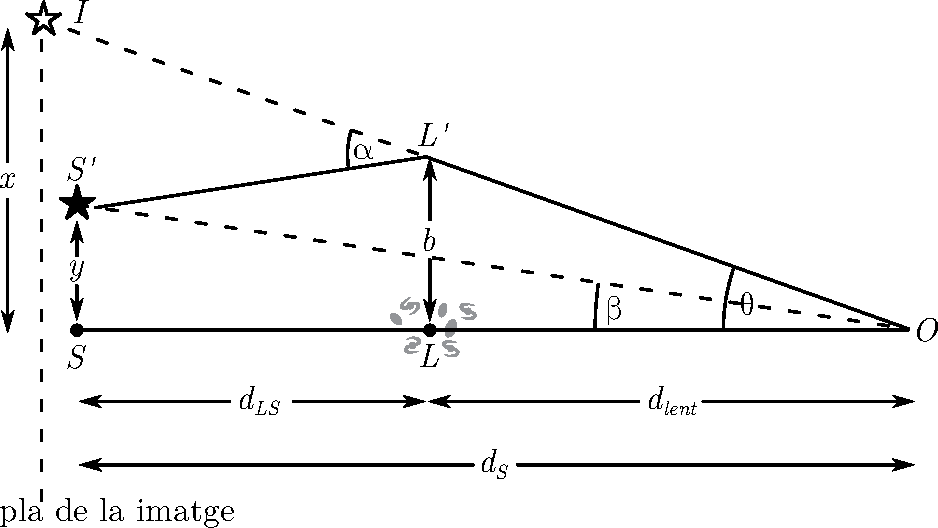
\includegraphics[width=0.75\textwidth]{./images/6-image-gravit}
	\caption{El camp gravitatori d'una massa puntual $M$ (situada a $L$) inclina la llum de l'estrella en $S'$ cap a l'observador. La impressió visual és que l'estrella es troba a $I$}
	\label{fig:image-gravit}
\end{figure}

Mitjançant \eqref{eq:alpha-deviation} es pot calcular la posició de la imatge $I$ si un objecte de massa $M$ s'interposa entre l'estrella $S$ i l'observador $O$ (figura \ref{fig:image-gravit}).

Si no hi hagués lent l'observador veuria l'estrella en $S'$, sota un angle $\beta \approx d_{S}$ (suposant que $y \ll d_{S}$). Ja que la llum s'ha desviat un angle $\alpha$, l'observador veu la imatge sota un angle $\theta \approx x/d_{S}$. Quan $\alpha \ll 1$, se segueix
\begin{align}\label{eq:xyalpha}
	x - y = \alpha d_{LS}
\end{align}
Dividint l'equació \eqref{eq:xyalpha} per $d_{S}$, i tenint en compte l'equació \eqref{eq:alpha-deviation}, suposant que $x \ll d_{S}$, i utilitzant $b \approx \theta d_{L}$, es troba
\begin{align}\label{eq:theta-beta}
	\theta - \beta = \frac{1}{\theta} \frac{4GM}{c^{2}} \frac{d_{LS}}{d_{L} d_{S}} \equiv \frac{\theta_{E}^{2}}{\theta}
\end{align}
on $\theta_{E}$ es coneix com \textit{radi d'Einstein} (tot i que en realitat és un angle).

L'equació \eqref{eq:theta-beta} es pot reescriure com
\begin{align}\label{eq:theta-einstein}
	\theta = \frac{1}{2} \qty[\beta \pm \sqrt{\beta^{2} + 4 \theta_{E}^{2}}]
\end{align}
Aquesta última expressió ens dóna la posició angular de la imatge en termes de l'angle $\beta$ i del radi d'Einstein.
\begin{itemize}
	\item Una estrella exactament darrere la lent ($\beta = 0$) es veurà com un cercle lluminós, al cel, de radi $\theta_{E}$.
	\item Si $\beta > 0$ (la imatge en $\theta_{+}$) apareixerà allunyada de la lent, amb $\theta_{+} > \beta$, fora del radi d'Einstein ($\theta_{+} > \theta_{E}$); aquestes imatges exteriors van ser les observades en torn al Sol eclipsat per la lluna.
	\item La imatge en $\theta_{-}$ és invertida i es troba dins el radi d'Einstein, al lloc oposat de la lent gravitatòria.
\end{itemize}
Tot i que les dues imatges produïdes ($I_{-}$ i $I_{+}$) poden confondre's en una sola (per ser les dues molt properes entre si), podem afirmar que una font lluminosa (estrella, núvol de gas, galàxia, cúmul, quàsar...) està sent afectada per una lent gravitacional (situada entre nosaltres i la font), si apareix més brillant.
\begin{itemize}
	\item Si la lent està en front d'una font extensa, una petita taca de llum al cel es convertirà en dues taques lluminoses en posar la lent entre la font i nosaltres. Les lents gravitacionals no afecten la lluminositat per unitat de superfície, de manera que la lluminositat aparent de cada imatge és proporcional a la seva àrea.
\end{itemize}

Sigui una regió angular $S'$ amb centre en la lent $L$, entre $y$ i $y + \Delta y$ (figura \ref{fig:amplif-lent}).
\begin{figure}[h]
	\centering
	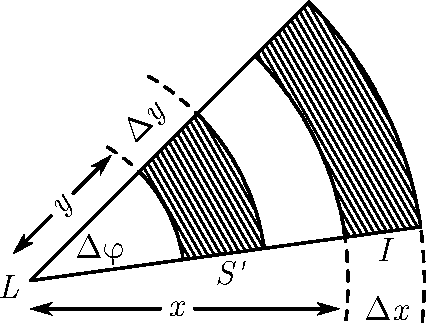
\includegraphics[width=0.35\textwidth]{./images/6-amplif-lent}
	\caption{Amplificació d'una imatge per una lent gravitacional}
	\label{fig:amplif-lent}
\end{figure}

Una imatge $I$ de $S'$ ocupa el mateix angle $\Delta \phi$ que $S'$, però les distàncies relatives al centre $L$ resulten ampliades o contretes:
\begin{align}
	\frac{x}{y} = \frac{\theta}{\beta} \Rightarrow \frac{\Delta x}{\Delta y} = \dv{\theta}{\beta}
\end{align}

En general, una imatge $S'$ més enllà de la lent $L$ resulta més brillant que la taca lluminosa original $S'$ (de no haver intervingut la lent). En canvi, una imatge més propera a l'observador que la lent $L$ resulta menys brillant.

El quocient de les àrees és
\begin{align}
	\frac{A_{imatge}}{A_{font}} = \abs{\frac{\theta}{\beta} \dv{\theta}{\beta}} = \frac{1}{4} \abs{\frac{\beta}{\sqrt{\beta^{2} + 4 \theta_{E}^{2}}} + \frac{\sqrt{\beta^{2} + 4 \theta_{E}^{2}}}{\beta} \pm 2}
\end{align}
de manera que la imatge $\theta_{+}$ és més brillant que la font $S'$, mentre que la imatge $\theta_{-}$ és menys brillant que la font llevat que $\beta < \theta_{E}/ \sqrt{2}$.

Conforme la lent (generalment invisible) es desplaça sobre el fons d'estrelles (pràcticament immòbil) el radi d'Einstein també es desplaça davant una estrella llunyana. Consegüentment veurem augmentar la lluminositat de l'estrella fins assolir un màxim i després decréixer.

Si aconseguim mesurar molts fenòmens de \textit{microlensing} i estudiar el moviment propi de la lent i de la font, la duració mitjana de l'augment en lluminositat ens dóna la massa de les lents gravitatòries. Si la lent consisteix en una estrella binària o en un sistema planetari els components del qual siguin tan propers entre ells que les regions dins dels radis d'Einstein se superposen, les corbes de llum resulten més complicades ja que es formen altres parells d'imatges i apareixen dos o més màxims de llum. En concret, per a una lent de $\SI{0.5}{\Msun}$ a una distància de nosaltres de $\SI{8}{\kilo\parsec}$, i amb una font a dues vegades aquesta distància, es troba que $\theta_{E} \approx \SI{5 e-4}{\arcsecond}$.

\subsubsection*{Objectes compactes massius de l'halo (MACHOs)}
Si suposem que la matèria fosca de l'halo de la Galàxia està constituïda per MACHOs, podrem calcular la probabilitat que una estrella distant sigui pròxima (en l'esfera celeste) a algun MACHO. Com que l'àrea de cada anell d'Einstein ($\pi d_{L}^{2} \theta_{E}^{2}$) és proporcional a la massa de la lent, la suma de totes les àrees només dependrà de la densitat numèrica de MACHOs i no de la massa individual de cadascun d'ells. Donada la massa fosca que es creu que existeix a la Galàxia, qualsevol estrella més enllà de la Galàxia tindrà una probabilitat de $\num{e-6}$ d'estar dins el radi d'Einstein d'algun MACHO. Així doncs, és necessari observar un milió d'estrelles llunyanes per tenir una probabilitat alta de veure alguna d'elles experimentar microlensing.

Una possible objecció a aquest procediment d'estimació observacional de la massa de MACHOs seria que l'augment transitori de lluminositat en una estrela llunyana podria ser degut no a microlensing, sinó a que aquesta estrella és polsant (e.g., una Cefeida). No obstant, en el cas d'estrelles polsants, la variació en lluminositat va acompanyada d'un canvi en temperatura i en color mentre que el microlensing no altera el color, ja que totes les longituds d'ona són afectades per igual pel camp gravitatori de la lent. Per aquesta raó els cercadors de microlensing mesuren la llum de les estrelles fent-les passar per dos filtres de diferents longituds d'ona. Només estrelles la lluminositat de les quals variï en la mateixa proporció en ambdós colors s'acceptaran com a candidats a microlensing.

Cap a l'any 2000 el MACHO Project hauria trobat entre 13 i 17 candidats a microlensing d'estrelles al Gran Núvol de Magalhães. La massa promig d'aquests candidats seria de $\SI{0.5}{\Msun}$ amb una fracció del 20\% de la massa de l'halo (amb un 95\% de confiança si el rang de masses està entre $\SIrange{0.15}{0.9}{\Msun}$, o bé entre $\SIrange{0.08}{0.5}{\Msun}$). Això suggereix que els MACHOs serien nanes blanques, però també podrien ser forats negres formats en transició quark--hadró, poc després del Big Bang.

%-----------------------------------------------------------------
\subsection[Partícules massives d'interacció feble]{Partícules massives d'interacció feble (WIMPs)}
L'estructura de l'Univers a gran escala ens indica que la major part de la matèria no és bariònica, ja que si no les fluctuacions de densitat de matèria en el desacoblament matèria--radiació (300 mil anys després del Big Bang) haurien donat lloc a anisotropies en la radiació de fons de microones molt majors que l'observació ens indica. Això ens diu, no obstant, de quin tipus de matèria no--bariònica es tracta.

L'escenari inicialment proposat, \textit{Hot Dark Matter} (HDM), a començaments dels anys 80, suposava que els WIPMs serien neutrinos, però aviat es va veure la incompatibilitat d'aquesta proposta amb la presència de matèria fosca en galàxies nanes (aquestes no poden retenir a aquests neutrinos donat el seu llarg lliure recorregut mitjà).

A mitjans dels anys 80 es va proposar \textit{Cold Dark Matter} (CDM). Aquest model va estar en voga aproximadament una dècada fins que es va veure la seva incompatibilitat amb les dades més recents d'estructures a gran escala ni amb la proporció de gas en cúmuls de galàxies.

A mitjans dels anys 90 van aparèixer models amb barreja de matèria calenta i matèria freda (CHDM), però aquests tenen dificultats en explicar l'abundància de cúmuls de galàxies. Per una altra banda, la radiació de fons de microones junt amb mesures de la quantitat de matèria present en l'Univers senyala clarament l'existència d'una component d'energia en forma de constant cosmològica (energia del buit) o bé d'un camp escalar.

Entre els diferents candidats a WIMPs en destaquen els neutrinos massius i els axions.

\subsubsection*{Neutrinos massius}
Experiments recents semblen indicar que el neutrino muònic tindria una massa superior a $\SI{0.5}{\eV}$, d'on aquests podrien contribuir amb un 0.5\% a la massa--energia total de l'univers.

Una altra possibilitat és que $m(\nu_{\tau}) \approx m(\nu_{\mu})$, això implicaria que els neutrinos contribuirien fins a un 20\% d'aquesta massa--energia.

Models de partícules elementals més enllà del model estàndard proposen l'existència d'un gran nombre de partícules (no incloses en aquest) de massa fins a $\SI{1}{\tera\eV}$. Tres candidats han estat suggerits:
\begin{itemize}
	\item El sneutrino (spin $= 0$).
	\item El gravitino (spin $= 3/2$).
	\item El neutralino (spin $= 1/2$).
\end{itemize}
D'entre ells, el més afavorit és el neutralino, la massa del qual podria estar entre $30$ i $\SI{60}{\giga\eV}$. De ser així, un continu flux de neutralinos provinents de l'halo de la Galàxia creuaria el nostre planera. D'aquí que hi hagi experiments em marxa orientats a detectar aquest flux.

\subsubsection*{Axions}
Aquestes partícules (també feblement interactives) tindrien masses en el rang de $\SIrange{e-6}{e-2}{\eV}$. Intents de detectar-les han fracassat fins el moment, però la seva base teòrica és tan sòlida que es confia en trobar-les tard o d'hora.

\subsubsection*{Detecció de WIMPs}
Com dèiem més anteriorment, existeixen intents de detectar el suposat flux de WIMPs conforme aquesta travessa la Terra segons aquesta recorre la seva òrbita en torn al Sol. El detector consisteix en $\ch{NaI}$ (iodur sòdic). La interacció d'una partícula WIMP amb un nucli del detector faria que el nucli experimentés un retrocés que es podria mesurar.
\begin{figure}[H]
	\centering
	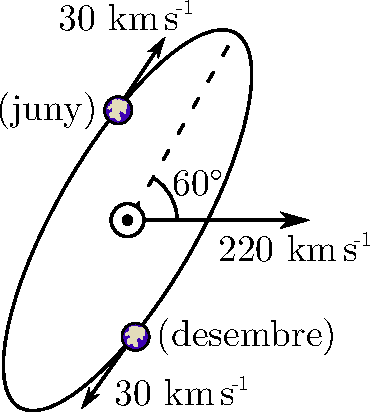
\includegraphics[width=0.25\textwidth]{./images/6-pla-terra-sol}
	\caption{La Terra orbita el Sol. Aquí es mostra la posició del nostre planeta al juny i al desembre}
	\label{fig:pla-terra-sol}
\end{figure}

La Terra orbita el Sol a $\SI{30}{\km\per\s}$ aproximadament, i el Sol orbita la Galàxia a $\SI{220}{\km\per\s}$. El pla de l'òrbita terrestre est 'a inclinat $\SI{60}{\degree}$ respecte al pla del disc de la Galàcia (figura \ref{fig:pla-terra-sol}).

Així és d'esperar que el flux de WIMPs sigui major al juny (quan la velocitat de la Terra i el Sol se sumen) que al desembre (quan es resten). La variació del flux entre ambdós mesos seria del 7\%.

L'experiment DAMA (\textit{Dark Matter Experiment}) sembla mostrar un senyal compatible amb aquestes característiques (figura \ref{fig:dama-results}). No obstant, aquests resultats no han estat corroborats per altres grups, els quals no mostren una variació significativa entre juny i desembre.
\begin{figure}[ht]
	\centering
	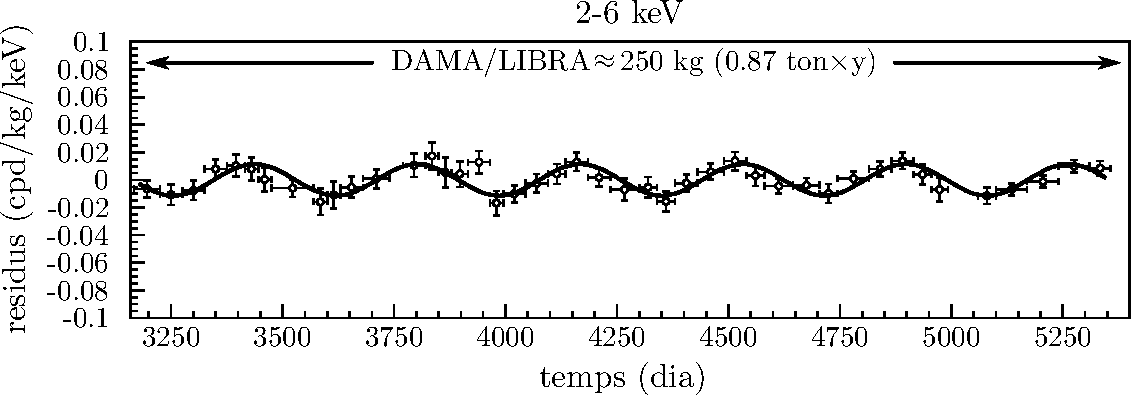
\includegraphics[width=0.9\textwidth]{./images/6-dama-results}
	\caption{Modulació del flux de partícules detectades a l'experiment DAMA en funció del temps}
	\label{fig:dama-results}
\end{figure}

Tanmateix, estan en marxa experiments encaminats a detectar WIMPs per mitjans indirectes. Així, l'anihilació de WIMPs en l'halo produiria un flux de raigs còsmics (integrals per protons i antiprotons). Globus sonda a gran alçada en l'atmosfera han detectat un excés de protons i antiprotons, però podria ser que aquests posseeixin un origen divers com la interacció de raigs còsmics primaris amb protons interestel·lars. L'anihilació de WIMPs podria també donar lloc a una radiació de fons de raigs gamma, amb una intensitat característica d'una ratlla $\gamma$ cap al centre de la Galàxia. El satèl·lit EGRET podria haver ja detectat aquest efecte.
